\def\year{2016}\relax
%File: formatting-instruction.tex
\documentclass[letterpaper]{article}
\usepackage{aaai16}
\usepackage[ruled,vlined,linesnumbered]{algorithm2e}
\usepackage{graphicx}
\usepackage{amsthm}
\usepackage{amsmath}
\usepackage{amssymb}
\usepackage{url}
\usepackage{times}
\usepackage{helvet}
\usepackage{courier}

\newcommand{\private}[2]{\textit{private}_{#1}(#2)}
\newcommand{\eff}{\textit{eff}}
\newcommand{\pre}{\textit{pre}}
\newcommand{\delete}{\textit{delete}}
\newcommand{\public}{\textit{public}}
\newcommand{\false}{\textit{false}}
\newcommand{\true}{\textit{true}}
\newcommand{\init}{\textit{init}}
\newcommand{\load}{\textit{load}}
\newcommand{\unload}{\textit{unload}}

\newtheorem{definition}{Definition}
\newtheorem{theorem}{Theorem}
\newcommand\cprivacy{object cardinality privacy}
\theoremstyle{definition}
\newtheorem{example}{Example}[section]

\frenchspacing
\setlength{\pdfpagewidth}{8.5in}
\setlength{\pdfpageheight}{11in}

\setcounter{secnumdepth}{0}
 \begin{document}
% The file aaai.sty is the style file for AAAI Press
% proceedings, working notes, and technical reports.
%
\title{Stronger Privacy Preserving Projections for Multi-Agent Planning}
\author{Shlomi Maliah \and Guy Shani \and Roni Stern\\\\
 Negev, Israel\\
}
\maketitle
\begin{abstract}
Collaborative privacy-preserving planning (CPPP) is a multi-agent planning task in which agents need to achieve a common set of goals without revealing certain private information. In many CPPP algorithms the individual agents reason about a {\em projection} of the multi-agent problem onto a single-agent classical planning problem.
For example, an agent can plan as if it controls the public actions of other agents, ignoring their unknown private preconditions and effects, and use the cost of this plan as a heuristic for the cost of the full, multi-agent plan. Using such a projection, however, ignores some dependencies between agents' public actions. In particular, it does not contain dependencies between actions  of other agents caused by their private facts. We propose a projection in which these {\em private dependencies} are maintained.
The benefit of our dependency-preserving projection is demonstrated by using it to produce high level plans in a new privacy preserving planner that is able to solve more benchmark problems than any other state-of-the-art privacy preserving planner.
This more informed projection does not explicitly share private information. In addition, we show that even if an adversary agent knows that an agent has some private objects of a given type (e.g., trucks), it cannot infer how many such private objects the agent controls. This introduces a novel strong form of privacy that is motivated by real-world requirements.
\end{abstract}
\section{Introduction}


%Designing autonomous agents able to act collaboratively as a team is a long standing goal in Artificial Intelligence. A fundamental aspect of such collaboration is the ability to plan for multiple agents acting in the world. In this work we address the problem of planning for multiple agents

% What is CPPP and why we care
{\em Collaborative privacy preserving planning (CPPP)} is a multi-agent planning task in which agents need to achieve a common set of goals without revealing certain private information. CPPP has important motivating examples such as planning for organizations that outsource some of their tasks and collaboration between military units where compartmentalization is required. CPPP recently received much attention
%~\cite{brafman2013complexity,nissim2014distributed,Brafman15,torreno2014aFlexible,maliah2014privacyPreserving,torreno2014fmap,torreno2015global,tovzivcka2014generating,jakubuv2015multiagent}
and new efficient solvers, scaling up to larger, more challenging domains, are constantly proposed~\cite[inter alia]{maliah2015privacy,nissim2014distributed,luis2014planMerging,tovzivcka2014generating,jakubuv2015multiagent}.




%\roni{This is very compressed and can be extended and improved}

% CPPP is nice, by single agent planning is much faster
%Even though research on CPPP is flourishing, classical planning algorithms are substantially more mature, offering very fast solvers with strong heuristics \cite{hoffmann2001ff,helmert2009landmarks}. An attractive approach, hence, is to {\em project} the multi-agent privacy preserving problem onto a classical planning problem, and employ a classical solver. Some planners use the resulting plan as a high-level plan for the individual agents to extend~\cite{tovzivcka2014generating,jakubuv2015multiagent,maliah2014privacyPreserving}, while other planners use the cost of that plan as a heuristic~\cite{nissim2014distributed}.

% view and projection
%Due to privacy, each individual agent has only a partial view of the world, containing its own private facts and actions, and its public actions. The agent also knows about the public actions of other agents, but is aware only of their public preconditions and effects. One can treat the agent view of the world as a classical planning problem, pretending that the agent controls the public actions of others. Then, one could solve this classical projection and obtain a plan.\roni{This repeats the above so I merged them}

% CPPP is nice, but single agent planning is much faster
Even though research on CPPP is flourishing, classical planners are substantially more mature, offering fast solvers with strong heuristics~\cite{hoffmann2001ff,helmert2009landmarks}. An attractive approach, hence, is to {\em project} the multi-agent problem onto a classical planning problem,  employ a classical solver, and then extend the resulting public plan using private actions~\cite{brafman2008one}.
%Some planners use the resulting plan as a high-level plan for the individual agents to extend~\cite{tovzivcka2014generating,jakubuv2015multiagent,maliah2014privacyPreserving}, while other planners use the cost of that plan as a heuristic~\cite{nissim2014distributed}.

% view and projection
Due to privacy, each individual agent has only a partial view of the world, containing its own public and private facts and actions. The agent also knows about the public actions of other agents, but is aware only of their public preconditions and effects. One can treat the agent view of the world as a classical planning problem, pretending that the agent controls the public actions of others. Then, one could solve this classical projection and obtain a plan.

%this projection is less than great
In this single-agent projection of the MA world, the agent is unaware of dependencies between other agents' public actions, originating from their private facts and actions. This results in an over optimistic assumption about agents' abilities. Take, for example, a blocksworld domain with two agents, where each agent controls a different arm, and conceals which block is held by the arm. The precondition of unloading a block $A$ on top of block $B$
by agent $1$ is that the agent is holding block $A$. As this is a private information, agent $2$ is unaware of this precondition, and thus believes that agent $1$ can put $A$ everywhere without picking it up.

%from agent i perspective the action - unstuck(A,B) of agent j that  puts block A on top of block B does, not contain the private precondition for holding A to begin with. Hence, agent i may believe that A can be put everywhere -by agent j- without picking it up.


% Without a good projection, we need to synchronize, which sucks
Thus, a solution to this single-agent projection is typically not a sound solution to the mulit-agent planning task, and some mechanism to communicate additional information is needed for constructing a sound plan. For example, in the MAFS algorithm~\cite{nissim2014distributed} agents broadcast partially encrypted states to all agents whenever a public action is performed. Methods of this type use a multi-agent planning mechanism, where all agents plan together, jointly revealing additional important information.

In this paper we take a different approach. We suggest a stronger projection, where all agents publish a projection of their private view of the world, containing only public actions. The joint projection is fed into a classical planner, resulting in a high level plan for achieving the goals, composed only of public actions~\cite{brafman2008one,maliah2014privacyPreserving}. Then, each agent extends the plan by adding private actions that allow it to accomplish its part in the public plan.

% Our approach: share the internal dependencies
The main drawback of the simple projection is the lack of information concerning dependencies between the public actions of an agent and between public actions and the initial state of the world.
Therefore, we focus on identifying these dependencies and sharing them in a privacy preserving manner. We define new facts that represent action dependencies, and explain when to add or delete these dependency facts.


The usefulness of the proposed projection is demonstrated in practice in a simple planner that uses a solution of the projected problem as a high-level plan, extending it to a full plan jointly by all agents. While the resulting planner is not complete, it is able to solve more benchmarks from the distributed multi-agent competition (CoDMAP)~\cite{vstolba2015competition} than any other state-of-the-art privacy preserving planner.

% But what about privacy??
Sharing the proposed projection between the agents does not violate the privacy requirement as the proposed projection does not contain any private information (fact or action) explicitly. This form of privacy is the current standard in the privacy preserving planning literature.
Another contribution of this work is the introduction of a more strict form of privacy that we call {\em \cprivacy }. This form of privacy addresses a realistic requirement in which agents are interested in hiding from other agents the number of private objects they control of specific types.

For example, a logistic company may wish to hide the number of trucks it controls, and the military would not disclose the number of bases in an area. An algorithm is said to preserve \cprivacy\ if an adversary, listening to the communication during planning, cannot distinguish between worlds where agents possess different quantities of private objects. We discuss the relationship between \cprivacy\ and other definitions of privacy, and show that our projection also preserves this type of privacy. %, that is, the projection is identical regardless of the number of private facts.

The contributions of this paper are hence two-fold: we provide the new definition of privacy -- \cprivacy -- and suggest a new strong projection, showing it both preserves \cprivacy\ and is key to the construction of a new planner to outperform existing state-of-the-art planners.

\section{Privacy Preserving Model}

\begin{figure}
\centering
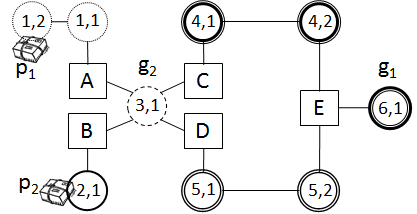
\includegraphics[width=\columnwidth]{Logistics}
\caption{A logistics example, where trucks deliver packages between logistics centers, denoted by squares. Each agent covers a set of cities, denoted by circles, and labeled $i,j$ where $i$ is the agent covering the city and $j$ is the local city index. The logistic centers can be entered by several agents, serving as collaboration sites.}
\label{fig:logistics}
\end{figure}


Research on privacy preserving planning focuses on variants of the multi-agent STRIPS model (MA-STRIPS)~\cite{brafman2013complexity} mainly due to its simplicity.


%We use here a multi-valued variables variant introduced recently by Brafman~\cite{Brafman15}.

%%%% STANDARD MV-MA-STRIPS definition %%%%%%%%%%%%
\begin{definition}[MA-STRIPS]
An MA-STRIPS problem is represented by a tuple $\langle P, \{A_i\}_{i=1}^k, I ,G \rangle$ where:
\begin{itemize}
	\item $k$ is the number of agents
%	\item $V$ is a finite set of finite-domain variables.
	\item $P$ is a finite set of facts (can be true of false).
%    \item For $1\leq i \leq k$, $A_i$ is the set of actions agent $i$ can perform.
    \item $A_i$ is the set of actions agent $i$ can perform.
	\item $I$ is the start state.
	\item $G$ is the goal condition.
\end{itemize}
\label{def:ma-strips}
\end{definition}
%The domain of a variable $v\in V$ is denoted by $dom(v)$.
%Each action $a=\langle pre,eff,c\rangle\in A=\cup_{i=1}^k A_i$ is given by its preconditions ($pre$), effects ($eff$), and cost ($c$).
Each action $a=\langle \pre(a), \eff(a), c(a) \rangle$ is defined by its preconditions ($\pre(a)$), effects ($\eff(a)$), and cost ($c(a)$). Preconditions and effects are logical formulas of $P$. A state is a conjunction of facts (true or false). The goal $G$ is also a conjunction of facts. The result of applying an action $a$ to a state $s$ is denoted by $a(s)$. A solution to a planning task is a {\em plan} $(a_1,\ldots,a_k)$ such that $G\subseteq a_k(\ldots(a_1(I)\ldots)$, i.e., a sequence of actions that transforms the initial state ($I$) to a state satisfying the goal condition ($G$).

%Preconditions and effects are partial assignments to of values to variables in $V$. A state is a complete assignment to all variables in $V$ and the goal condition $G$ is a full or a partial assignment of values to variables in $V$. The result of applying an action $a$ to a state $s$ is denoted by $a(s)$. A solution to a planning task is a {\em plan} $\pi=(a_1,\ldots,a_k)$ such that $G\subseteq a_k(\ldots(a_1(I)\ldots)$, i.e., it is a sequence of actions that transforms the initial state ($I$) to a state that satisfies the goal condition ($G$).


Figure~\ref{fig:logistics} illustrates a simple logistic example in which the agents are trucks tasked with delivering packages. %The variables $V=\{p1\_at, p2\_at, t1\_at, t2\_at, t3\_at, t4\_at, t5\_at, t6\_at \}$,
The set of facts $P$ represents the location of the two packages and the six trucks. Each truck has three actions: move, load, and unload, corresponding to moving the truck between locations, loading a package and unloading it. Trucks can only drive along the edges in Figure~\ref{fig:logistics}. Agents are heterogeneous  and their range is restricted, such that location $i,j$ can only be reached using truck $i$. The rectangles are logistic centers visited by multiple trucks that load or unload packages.

\subsection{Privacy}

Privacy-preserving MA-STRIPS extends MA-STRIPS~\cite{brafman2008one} by defining sets of variables and actions as private, known only to a single agent. Let $\public(P)$ be a set of public facts, whose value is always known to all agents. Let $\private{i}{P}$ be a set of facts whose existence and value is known only to agent $i$. Each agent has a set of actions it can execute, where $\private{i}{A}$ is a set of private actions, that no other agent knows about, and their execution is hidden from other agents, and $\public_i(A)$ is a set of public actions. A private action can have only private effects. A public action may have both public and private effects. Upon the execution of a public action, all agents observe its public effects. For ease of exposition we assume that all goals are public, although our method can be extended to handle private goals.

A solution to a privacy-preserving MA problem, is a sequence of public and private actions. We say that the sequence of public actions in such a solution is a {\em valid} high-level plan if it can be extended to a full plan using the agents' private actions.

Extending a valid high-level plan to a full plan can be done by all agents concurrently, where each agent plans independently to achieve the preconditions of its actions in the high-level plan~\cite{maliah2014privacyPreserving}.

% Local view of a public action
Consider a public action $a$ of agent $j$ from the perspective of agent $i$.
The action is public, so agent $i$ knows about $a$'s existence. However, if $a$ has private preconditions and effects, they are only known to agent $j$ and are hidden from agent $i$. Formally, we define the {\em local view} of action $a=\langle \pre(a),\eff(a),c(a) \rangle$ by agent $i$, denoted $\pi_i(a)$, as
\[ \pi_i(a)=\langle \public(P)\cap \pre(a), \public(P)\cap \eff(a), c(a) \rangle \]
Clearly, $\pi_i(a)=a$ if $a$ is an action of agent $i$.



\begin{definition}[Local View]
%The {\em local view} of agent $i$ of an MA-STRIPS problem $\pi=\langle  P, \{A_i\}_{i=1}^k, I ,G \rangle$
Given an MA-STRIPS problem $\pi=\langle  P, \{A_i\}_{i=1}^k, I ,G \rangle$,
the {\em local view} of agent $i$ is defined by the tuple
$\pi_i=\langle
\pi_i(P), \{\pi_i(A_j)\}_{j=1}^k,\pi(I),\pi(G)
\rangle
$
where:
\begin{itemize}
\item $\pi_i(P)=\public(P)\cup \private{i}{P}$
\item $\pi_i(I)=I \cap \pi_i(P)$
\item $\pi_i(G)=G \cap \pi_i(P)$
\end{itemize}
\label{def:local-view}
\end{definition}



In our running logistic example, assume now that each truck is owned by a different company, and that one company does not want to share its location and coverage (which locations it can reach) with other companies.
The only actions that are public are load/unload actions from/at logistic centers. The only facts that are public are facts representing whether a package is at one of the logistic centers. Load/unload actions from/at private locations and all move actions are private actions. The location of the trucks, and facts representing whether a package is at one of the private locations, are all private facts.
%Thus, all the facts representing the location of trucks are private, while the facts representing whether a package is at a logistic center are public. Only the load/unload actions at the logistic centers are public, and load/unload private locations and all move actions are private to each agent.
The local view of agent 3 consists of the facts representing
packages at $A$, $B$, $C$, $D$, $E$, and (3,1);
%which packages are at the logistic centers or package locations,
the facts representing possible locations of truck $3$;
the move, load, and unload actions of truck $3$;
and the load/unload actions of all agents from/to logistics centers.
For example, the local view of a load action of another agent has a precondition regarding the location of the package only, ignoring the private precondition of the location of the truck.





\begin{definition}[Privacy-Preserving MA-STRIPS]
A privacy-preserving MA-STRIPS problem is defined by an MA-STRIPS problem and the $\public(\cdot)$ and $\private{i}{\cdot}$ functions for every $i\in[1,n]$. The task is to find a solution without revealing private information during planning.
\label{def:private-ma-strips}
\end{definition}

In Section~\ref{sec:preserving} we discuss concrete definitions for private information that must not be revealed during planning.


\section{Classical Projections and Regression}

We now discuss projections of a privacy-preserving multi-agent problem into classical single-agent planning, and the regression of formulas through action sequences, both of which are key concepts in our projection algorithm.

\subsection{Classical Projections}


% What is a single-agent projection and a complete single agent projection
A {\em classical projection} of a privacy-preserving multi-agent problem is a compilation of the problem into a classical single-agent problem. For example, one can consider the local view (Definition~\ref{def:local-view}) of the agent as a classical planning problem, pretending that the agent controls the public actions of other agents as well.

A classical projection is {\em sound} if the sequence of public actions in any solution to the projected problem, can be extended using only private actions  to a solution to the original multi-agent problem. As efficient privacy preserving projections tend to be lossy, not capturing all the information in the original problem, achieving soundness is difficult.

We say that a classical projection is {\em complete} if given a solution to the original privacy preserving problem, there exists a solution to the projected planning problem with the same sequence of public actions. An example of a complete classical projection is the local view projection.

% Why complete single-agent projection is helpful

%A complete classical projection can therefore at least provide a heuristic for solving the original problem \cite{nissim2014distributed}. Moreover, some privay preserving algorithms use the solution to the projected planning problem as a high level plan and try to extended it to a complete plan by adding private actions of the individual agents~\cite{jakubuv2015multiagent,tozicka2015internally}.
Classical projections are of interest because they can be solved by each agent, providing a heuristic estimation for the cost of solving the original problem \cite{nissim2014distributed}. Moreover, some privacy preserving algorithms use the solution to the projected planning problem as a high level plan and try to extended it to a complete plan by adding private actions of the individual agents~\cite{jakubuv2015multiagent,tozicka2015internally}.


%For example, one can consider the local view of the agent as a single agent problem, assuming that the agent controls the public actions of other agents as well.

%A helpful property of the local projection for agent $i$ is that it is complete, in that any solution to the MA-STRIPS problem must be a solution to the local projected problem. Thus, solving a local projection provides at least a heuristic for solving the original problem \cite{raz}, and in many cases it provides a skeleton of a solution that can be extended by the individual agents to a complete solution.



% Limitations of a local view projection
\subsubsection{Dependencies}

While a local view of an agent is a complete single-agent projection, it fails to consider some dependencies between public actions of another agent. In particular, the local view of agent $i$ contains no information about {\em private dependencies} of other agents' public actions. %, defined as follows.

%In particular, the local view of agent $i$ contains no information about {\em private dependencies} between public actions of agent $j$ or dependencies between public actions of agent $j$ and private facts in the initial state.

\begin{definition}
A public action $a$ {\em facilitates} the achievement of a private fact $f$, if $f$ is an effect of $a$, or there exist a sequence of private actions $a_1,...,a_k$ such that:
\begin{itemize}
\item $f$ is an effect of $a_k$,
\item each $a_i$ takes as precondition an effect of some $a_j$ s.t. $j<i$,
\item $a_1$ takes as precondition an effect of $a$.
\end{itemize}
\end{definition}

\begin{definition}[Private Dependency]
An action $a$ is said to have a private dependency if it has a private fact $f$ as a precondition such that one of the following hold: (1) there is another public action $a'$ that facilitates achieving $f$,  (2) $f$ is either true in the start state or can be achieved from it by only applying private actions. We call the first type of private dependency an action-to-action dependency and call the second type an init-to-action dependency.
%An agent $i$ is said to have a private dependency if one of the following hold: (1) Agent $i$ has two public action $a,a'\in public(A_i)$ such that $a$ has a private fact $f$ as a precondition, and executing $a'$ facilitates achieving $f$.  (2) Agent $i$ has a public action $a\in \public(A_i)$ that has a private fact $f$ and that fact can be privately achieved from the initial state. We call the first type of private dependency an action-to-action dependency and call the second type an action-to-init dependency.
\label{def:private-dependency}
\end{definition}

%These private dependencies arise when executing a public action $ has a private fact as a precondition, and either (1) that precondition is part of the initial state, creating a depending , or that in order to achieve this precondition the agent must perform some other public action, thus creating
%and that private facts is either part of the initial state or executing another public action is needed to
%that is either an effect of someprivate effect that is later needed in order to execute another public action, or (2) the initial state contains a private fact that is later needed to execute a public action.

%For example, the public {\em (load p t B)} action provides a private effect {\em (on p t)}, that is later needed by the public {\em (unload p t A)} action. Thus, {\em (unload p t A)} has a private dependency of the type ``action-to-action''.
In our logistic example (Figure~\ref{fig:logistics}), the public action {\em (unload p t3 A)} has a private precondition {\em (on p t3)},
and the public action {\em (load p t3 B)} achieves it. Thus, {\em (unload p t3 A)} has a private dependency of the type ``action-to-action''.
%Thus, {\em (unload p t A)} these two actions have a private dependency between them (of the ``action-to-action'' type).
The local views of the other agents do not include this private dependency: the public {\em (unload p t3 A)} action
will appear in the local views of all agents (except agent 3) without the precondition {\em (on p t3)}, since it is a private fact. As a result, agents will believe that unloading a package at arbitrary public locations is always possible.
As an example of an ``action-to-init'' private dependency, consider the public action {\em (unload p2 t2 B)}, which has a private precondition
{\em (on p2 t2)}. This precondition can be achieved by a private action {\em (load p t2 (2,1))}, which in turn require the private fact {\em (at p2 B)}, which is true in the initial state. All agents (except agent 2) do not know about this precondition of {\em (unload p2 t2 B)} and would assume that t2 can always unload p2 at B, even if p2 was already moved beyond the reach of t2.
In this work we suggest a stronger projection where information about private dependencies is shared, based on the concept of {\em regression}. %, described below.
% TODO-R: Make above sentence prettier


%\roni{Add a connecting line}


%However, this projection is clearly very partial, as it fails to consider any private dependencies between public actions of other agents. For example, the projection of the {\em unload p t A} action, which has private preconditions {\em (at t A)} and {\em (on p t)}, has no precondition in the projection. Agents may hence believe that unloading a package at arbitrary locations is always possible.
%\item Thus, projections have been used ads a heuristic


\subsection{Regression}
% Intuition of what is a regression
Regression is a fundamental tool in automated planning, in which we seek the conditions needed to reach a state, achieve a fact, or perform an action. More generally, if a formula $\phi$ describes a constraint on state facts and $a$ is an action then the regression of $\phi$ through $a$, denoted $rg_a(\phi)$, is a formula that describes the minimal constraints on state facts such that if we apply $a$ to a state that satisfies $rg_a(\phi)$ we will reach a state  that satisfies $\phi$.


% Formal
In the context of classical planning, Rintanen \shortcite{Rintanen} describes how to compute the regression of a formula $\phi$ through an action $a$. We now review these definitions.


For ease of exposition, we assume here that both the effect and the precondition of an action are conjunctions of literals. That is, we do not allow conditional effects or disjunction of preconditions. We assume that the initial state is induced by an $init$ action, which assigns to all predicates their value at the initial state of the problem. The $init$ action can only be applied once and has no preconditions. We also assume that both the preconditions and effects of all actions are consistent, e.g., for a given literal $l$, no effect or precondition contains both $l$ and $\neg l$. These are not real restrictions, and we could use Rintanen's full regression definition at the cost of a more complicated exposition. %explanation of our methods.

In this restricted representation, Rintanen's regression of a formula $\phi$ through an action $a$, defined only over a single literal or a conjunction of literals, is simplified as follows: %\roni{Why ``simplified''?} \guy{Because the original Rintanen definition with conditional effects is much more complex}:
\begin{definition}[Regression]
%The regression function $rg_a(\cdot)$ is defiend as follows:
\begin{align}
&rg_a(l)=  \pre(a)  :  l \in \eff(a)&\\
&rg_a(l)= false   :  \exists l' \in \eff(a) \mbox{ s.t. } l,l' \mbox{ are mutex}&   \label{eqn:mutex}\\
&rg_a(l)= l  :  l,\neg l \not\in \eff(a)&\\
&rg_a(\phi)=  \bigwedge_{l \in \phi} rg_a(l)  :  \phi = l_1 \wedge l_2 \wedge ... \wedge l_k &
\end{align}
\label{def:regression}
\end{definition}
 Rintanen shows that if $s \models rg_a(\phi)$ then $a(s)$ satisfies $\phi$.

% A regression tree
Given a set of actions $A$, we define the regression tree of a conjunction formula $\phi$ using actions in $A$, denoted $T_{rg}(\phi, A)$.
Intuitively, the regression tree of $\phi$ represents all possible
sequences of regression functions $rg_a(\cdot)$ that can be applied to $\phi$, i.e., all sequences of actions in $A$ that achieve $\phi$.
The nodes of the regression tree are labeled by formulas (given our restricted action definition, these formulas are only conjunctions of literals), and the edges are labeled by actions. We denote the formula associated with node $n$ by $n.\phi$. The set of outgoing edges of a node $n$ are labeled by all actions $a \in A$, s.t. $\exists l \in n.\phi : l \in \eff(a)$. That is, all actions that provide at least one literal in $n.\phi$.

Algorithm~\ref{alg:regression} shows the construction of the regression tree. The tree is constructed top down, starting from the root. Leaves are labeled by either $true$ or $false$. Every sequence of edges in every path from a $true$ leaf to the root in the regression tree corresponds to a plan that achieves $\phi$ --- the formula at the root of the tree. During the construction of the tree,
we may reach a node $n$
that has an ancestor node $n'$ for which $n.\phi \models n'.\phi$.
%*********************************************$.
% BEFORE ANY OF US CHANGES THE \MODELS DIRECTION ONE MORE:
% Here's an example:
% 1. Let n be on(a,b) and on(b,c).
% 2. Let n' be on(a,b)
% 3. We do not want to regress from n if it has a parent n'.
% 4. So the rule should be halt if n \models n'
% i.e., halt if a node entails one of its parents.
%*********************************************$.
This means a cycle has been identified in the regression tree, and we need not further develop $n$. To remove the cycle, we set $n.\phi$ to $false$.
% TODO-R: Say that this is to make the regression tree be a compact representation of how to achieve \phi

\begin{algorithm}[b!]
\small
	\SetKwBlock{Regress}{Regress($\phi$, $A$)}{end}
\Regress{
	\KwIn{$\phi$, a conjunction of literals}
    \KwIn{$A$, a set of actions to regress with}
	\KwOut{$n$, the root of the regression tree}
    $n \leftarrow$ a tree node\\
    \lIf{$\phi=\false$}{\Return $\false$}
    \ForEach{ancestor $n'$ of $n$}{
    	\If{$\phi \models n'.\phi$}{
        	$n.\phi \leftarrow \false$\\
            \Return $n$\\
        }
    }
    \If{$\phi$ is not empty}{
      $n.\phi \leftarrow \phi$\\
      \ForEach{action $a$}{
          \If{$\eff(a) \cap \phi \neq \emptyset$}{
%              $n_a \leftarrow Regress((\phi\setminus \eff(a))\cup \pre(a), A)$\\
%              $\phi_a \leftarrow rg_a(n.\phi)$\\
			  $n_a \leftarrow Regress(rg_a(n.\phi),A)$\\
              Add $n_a$ to $n.children$\\
          }
      }
	}
    \Else{
    	$n.\phi \leftarrow \true$\\
    }
    \Return $n$   \\
}
\caption{Computing the regression tree $T_{rg}(\phi,A)$ for a conjunction of literals $\phi$ with a set of action $A$}
\label{alg:regression}
\end{algorithm}



%\section{Solution Approach}
%\begin{itemize}
%\item Following the GPPP approach: plan public actions/effects, then ground them
%\item Compiling the
%\item Levels of privacy
%\end{itemize}

%\section{Strong Projection using Inter-Action Dependencies}%Compiling Away Private Facts and Actions}
\section{Dependency-Preserving Projection}

We now present our novel projection, which we call the {\em dependency-preserving projection} (DP projection). DP projection shares private dependencies without explicitly sharing private information. Unlike the local view projection, a DP projection is generated by all agents collaboratively, either sequentially, one agent at a time, or in parallel.

Intuitively, the DP projection contains all public facts, and replaces every public action $a$ with a set of actions, $\alpha(a)$, where each action in $\alpha(a)$ represents executing $a$ after a set of public actions that enable achieving $a$'s private preconditions.
% Every action $a_b$ in $\alpha(a)$ represents executing $a$ after a set of public actions $A_b$ were executed to enable achieving $a$'s private  preconditions. % \roni{What about the public preconditions? aren't they regressed as well?}
More formally, let $A_b$ be a set of public actions that facilitates the achievement of all private preconditions of a public action $a$. For each such set we create an action $a_b$, whose preconditions ensure that $a$ is executed after the execution of all actions in $A_b$. The set $\alpha(a)$ is composed of all such actions $a_b$.

Ensuring that $a$ is executed only after all actions in $A_b$ is done by maintaining a set of facts $f_{a'}$ for every public action $a'$, which is true if the effects of $a'$ were achieved. Thus, the projection $\pi_{DP}$ consists all public facts in $\pi$, a public fact $f_a$ and a set of actions $\alpha(a)$ for every public action $a$.

Next, we present and explain the exact details of how each agent generates appropriate $\alpha(a)$ actions from its local view. The conjunction of the projected actions and facts by all agents produces the complete DP projection.


%This is done by considering its local view and  a special form of regression trees


%, analyze their local views and add information that is used to construct the DP projection.

%both public and  private dependencies between actions, without explicitly sharing private information.

%Section~\ref{sec:preserving} discusses the loss of privacy due to sharing this dependency information.
%Intuitively, DP projection captures the private relationships between public actions of an agent $i$, that is, which public actions of $i$ should be executed to enable other public actions of $i$. The public dependencies through the public facts are maintained in the projection.
%We now explain in detail the construction of the DP projection.

%The key insight in the development of the DP projection is that we add actions and facts to the project that define explicitly the dependency between a public action $a$ and the set of public actions that enabled performing $a$.
%The key insight in the development of the DP projection is that we add ``artificial'' public facts to keep track of which public actions have been performed, and  that define explicitly the dependency between a public action $a$ and the set of public actions that enabled performing $a$.



%In addition, for each public action $a$ of agent $i$, a DP projection includes a set of actions $\alpha(a)$, each representing a possible sequence of public and private actions taken prior to executing $a$. A DP-projection also includes a set of dependency facts $\delta(a)$, representing the dependency of $a$ on other public actions in these sequences. Note that no private action or fact appears in this projection.
%\roni{There is no clear definition of what is $\delta(a)$}\guy{check if this is better now}
%The private actions and facts of the agents do not exist in the projection.

% SHLOMI'S TEXT: foreach action a we create a set of projection actions alpa(a) that contain alternative actions of a. Each of the action from alpa(a) has a identical effect as action a and it present by its preconditions the dependency of action a on unique public action set. we also define a set of facts gama(a), that representing the dependencies of a on the execution of others public action.



\subsection{Creating the Regression Tree}


% We run regression on the local planning problem (as define by the PSM guys)
%For a public action $a$ of agent $i$, we use regression to identify sequences of private and public actions of $i$, as well as public actions of other agents, that enable the agent to execute $a$. Each of these sequences will be mapped to an action in $\alpha(a)$, which will then be added to $\pi_{DP}$.
For a public action $a$ of agent $i$, we use regression to identify unique sets of public actions of $i$ that enable the agent to execute $a$. Each of these sets of actions will be mapped to a single action in $\alpha(a)$ and added to $\pi_{DP}$.
In more details, we construct a regression tree for $\pre(a)$ over a slightly revised local view of agent $i$ in which all public actions (except for $a$) have no preconditions. This revised local view (denoted $\pi_i^r$) is used instead of agent $i$'s local view ($\pi_i$) because in constructing $\alpha(a)$ we do not model the conditions required for executing other public actions. Rather, $\alpha(a)$ models how other public actions enable executing $a$.


Specifically, $\pi_i^r$ is equal to $\pi_i$ except that every public action $a_p$ in $\pi_i$ is replaced by a revised action $a^r_p$:
% TODO-R: change "local view of a public action"
%explained below.\roni{why do we need a revised local view?}\guy{we use a revised version in order to keep the regression algorithm standard. Another option would have been to keep the local view as is and modify the algorithm. I think that it is cleaner as is.}\roni{While I disagree in terms of what I think is clearer to the reader, I did not change it and followed your lead} Instead of using the existing public actions in the regression tree creation, we replace each public action with a revised version, that has no preconditions. Thus, we do not model the conditions required for the execution of pubic actions other than $a$, but rather how these public actions help us to execute $a$.  Specifically, let $a_p$ be a public action of agent $i$, or a local view of a public action of another agent. The revised action $a^r_p$ of $a_p$ is defined as:
\begin{eqnarray}
& \pre(a^r_p)=true &\\
%& \eff{a^r_p}=\displaystyle\bigwedge_{l \in \eff{a_p}}l \bigwedge_{l' \in pre(a_p), \neg l' \not\in \eff{a_p}}l'&
& \eff(a^r_p)=\displaystyle\left(\bigwedge_{l \in \eff(a_p)}l\right) \wedge \left(\bigwedge_{l' \in \pre(a_p), \neg l' \not\in \eff(a_p)}l'\right)&
\end{eqnarray}
That is, $a^r_p$ has no preconditions and has the effects of $a_p$.
In addition, the preconditions of $a_p$ are added to the effects of $a^r_p$ if they are not deleted by $a_p$ as these facts must be true after $a_p$ was executed.
This captures the state of the world immediately after $a_p$ was executed. Consider, for example, an action $a$ with precondition $p$ and effect $q$. Immediately after $a$ was executed, $(p \wedge q)$ must hold. Furthermore, this process helps us in detecting conflicts between public actions, as we later show in Example~\ref{ex1}.


Every agent $i$ uses the set of revised actions $\pi_i^r.A$ to construct a regression tree for every action $a$ by calling Algorithm~\ref{alg:regression} with parameters $\pre(a)$ and $\pi_i^r.A$. For brevity, we will denote the resulting regression tree as $T_{rg}(a)$. The branches of $T_{rg}(a)$ ending at leaves labeled by $true$ represent plans to achieve the precondition of $a$, taking into consideration agent $i$'s local view and assuming that other agents' public actions can always be executed.


%using its private actions, and the revised version of the public actions of $i$ as well as the revised public actions of other agents.
%The branches of the tree ending at leaves labeled by $true$ represent plans to achieve the precondition of $a$, assuming that other public actions can always be executed.



\begin{figure}
\centering
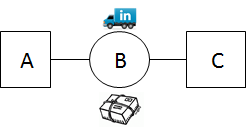
\includegraphics[scale=0.7]{SmallLogistics}
%\caption{A smaller logistics example domain of a single agent. Locations $A$ and $C$ are logistics centers, and $B$ is a private city. A truck $t$ and a package $p$ are initially at $B$.}
\caption{A simple logistics example.}
\label{fig:small}
\end{figure}


\begin{figure}
\centering
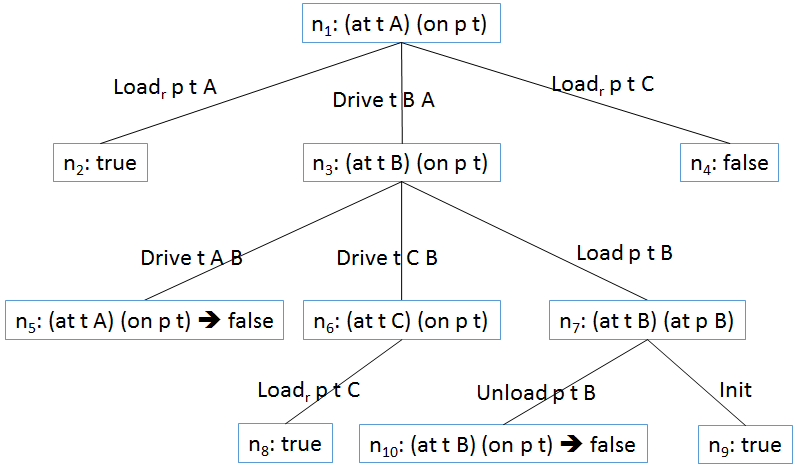
\includegraphics[width=\columnwidth]{RegressionTree}
\caption{Partial regression tree for {\em (unload p t A)} in Fig.~\ref{fig:small}.}
\label{fig:tree}
\end{figure}


\begin{example}
\label{ex1}
Let us look at the smaller logistics example in Figure~\ref{fig:small}, where an agent has one private city $B$ and two public logistic centers $A$ and $C$. Figure~\ref{fig:tree} shows the regression tree constructed for  action {\em (unload p t A)} with precondition {\em(at t A)} and {\em(on p t)}. %Recalling that the revised action $load_r$ for the public {\em load p t A} action has the precondition $true$ and effect {\em (on p t) (at t A)}, we can see that
As the revised action $load_r$ for the public {\em load p t A} action has the precondition $\true$ and effect {\em (on p t) (at t A)}, regressing through this action results in the $\true$ formula at node $n_2$. On the other hand, due to the conflict between {\em (at t A)} and the effect {\em (at t C)} of the revised action for {\em (load p t C)}, the regression result is $\false$ for node $n_4$ (following rule~\ref{eqn:mutex} in Definition~\ref{def:regression}). $n_5.\phi$ is satisfies the formula at $n_1$, and is hence replaced by $\false$, denoting a cycle. The same holds for $n_{10}.\phi$, which satisfies $n_3.\phi$. The $\true$ leaves of the tree correspond to the plans {\em (load p t C), (drive t C B), (Drive t B A)},  {\em (\init), (\load\ p t B), (Drive t B A)}, and {\em (\load\ p t A)}.
\end{example}

\subsection{Creating Projected Actions}

Using the regression tree described above, we can finally generate for a public action $a$ of agent $i$ the set of actions $\alpha(a)$ that will be added to the DP projection instead of $a$. Next we describe how $\alpha(a)$ is constructed.

Recall that every branch $b$ in $T_{rg}(a)$ from a leaf $n$ where $n.\phi=\true$ to the root represents a plan for achieving $\pre(a)$.
Every such a branch $b$ is mapped to a set of public actions $A_b$, which are all the public actions in $b$ that achieve a private precondition for another action in $b$. For every set of public actions $A_b$ we add a single action $a_b$ to $\alpha(a)$. Executing $a_b$ is intended to represent executing $a$ after the actions in $A_b$ have been executed. Thus, the preconditions of $a_b$ must verify that the actions in $A_b$ were executed.

%, representing executing $a$ after $A_b$ was executed. %the set of public actions that achieve a private fact in $b$ were performed. %that appear in the corresponding plan were achieved.



%Let $a_b\in \alpha(a)$ be an action added to $\alpha(a)$ for a set of public actions $A_b$. Executing $a_b$ is intended to represent executing $a$ after the actions in $A_b$ have been executed. Thus, the preconditions of $a_b$ must verify that the actions in $A_b$ were executed.
To keep track of which public actions have been performed so far, we define a fact $f_{a'}$ for every action $a'\in A_b$. There is a single fact for every public action, used in all occurrences of $a'$ in $\alpha(\cdot)$ of all agents. We also add a fact $f_{init}$, representing the execution of the $init$ action.

The preconditions of $a_b$ are the public preconditions of $a$
in conjunction with $\bigwedge_{a' \in A_b}f_{a'}$.
The add effects of $a_b$ are the effects of $a$ in conjunction with setting $f_a$ to be true, allowing other actions that depend on the execution of $a$, to be executed. We discuss the delete effects of $a_b$ later on.
Throughout the rest of this paper, we refer to actions in $\alpha(a)$ as {\em projected actions} and refer to the added facts $f_{a'}$ as {\em dependency facts}.

%Let $a_b$ be an action added to $\alpha(a)$ that represents the set of public actions $A_b$. The precondition of $a_b$ contains the public preconditions of $a$, in conjunction with $\bigwedge_{a' \in A_b}f^{a'}_a$, representing that executing these public actions enables achieving some private precondition of $a$. Let $\beta(a)$ be the dependency facts $f^a_{a'} \in \delta(a')$ over all $a'$, capturing the dependency of other actions $a'$ on $a$. The effect of every action in $\alpha(a)$ is the public effects of $a$, as well as $\bigwedge_{f \in \beta(a)} f$.



Note that the same set of public actions may appear in different branches of the regression tree, possibly in different orders. Thus, multiple branches may be represented by a single action in $\alpha(a)$.
We intentionally group branches that have the same set of public actions and do not add a projected action for every branch in $T_{rg}(a)$ for privacy reasons. Imagine, for example, that a logistics agent can transfer a package from public location $A$ to public location $B$ in two possible routes, each passing through a different sequence of private locations, and thus, resulting in two different sequences of private and public actions. If the agent published two different projected actions, each corresponding to a different route, then the other agents would learn that the agent surely covers more than a single private location, thus revealing private information.



%For each public action $a$, we create a set of projected actions $\alpha(a)$, each corresponding to a sequence of public and private actions ending with $a$. In addition, we define a set of facts $\delta(a)$, each representing a dependency of $a$ on a public action appearing in these sequences. We now explain the construction of $\alpha(a)$ and $\delta(a)$ using the regression tree $T_{rg}(\pre(a))$.
%An action $a_{\{a_1,...,a_k\}}\in \alpha(a)$ represents the execution of $a$ after the public actions $a_1,...,a_k$ were already executed.
%To only add sets of actions that correspond to actual plans that achieve facts needed for the execution of $a$, we generate an action $a_{\{a_1,...,a_k\}}\in \alpha(a)$ only for sets of actions that consists a complete branch in the regression tree of $a$ that ended with leaf
%$n$ where $n.\phi=\true$. This is because each branch $b$ in the regression tree from a leaf $n$ where $n.\phi=\true$ to the root represents a plan for achieving $\pre(a)$.

%For each such set of actions $A_b$ we construct a projected action $a_b$ and add it into $\alpha(a)$. The precondition of $a_b$ contains the public preconditions of $a$, in conjunction with $\bigwedge_{a' \in A_b}f^{a'}_a$, representing that executing these public actions enables achieving some private precondition of $a$. Let $\beta(a)$ be the dependency facts $f^a_{a'} \in \delta(a')$ over all $a'$, capturing the dependency of other actions $a'$ on $a$. The effect of every action in $\alpha(a)$ is the public effects of $a$, as well as $\bigwedge_{f \in \beta(a)} f$.

%A dependency fact $f^{a'}_a \in \delta(a)$ represents the dependency of $a$ on the execution of another public action $a'$.

%We focus on public actions of agent $i$ that appear along some branch from a node labeled by $\true$ to the root, supplying some private fact required for enabling a precondition of $a$. For each such public action $a'$, we introduce a new fact $f^{a'}_a \in \delta(a)$, representing the dependency of $a$ on the execution of $a'$. As $\init$ may also appear along some branch, we can also have facts $f^{\init}_a \in \delta(a)$, representing the dependency of $a$ on the initial state.

%Each branch $b$ from a leaf $n$ where $n.\phi=\true$ to the root represents a plan for achieving $\pre(a)$.
%We are interested in the set of public actions $A_b$ that appear along the branch $b$ from a leaf $n$ to the root ($\pre(a)$), achieving at least one private fact during the regression. The same set of public actions may appear in different branches of the tree, and we ignore such duplicates for privacy reasons. Imagine, for example, that a logistics agent can transfer a package from public location $A$ to public location $B$ in two possible routes, each passing through a different sequence of private locations, and thus, resulting in two different sequences of private and public actions. If the agent published two different projected actions, each corresponding to a different route, then the other agents would learn that the agent surely covers more than a single private location, thus revealing private information.
%\roni{This is very obscure. What are the privacy reasons? why would this discover private information?}\guy{hope that this is better.}




\subsection{Removing Consumed Dependencies}
\label{sec:removingConsumed}
Let $a_b$ be a projected action and let $b$ be a plan in the regression tree that generated $a_b$ (i.e., the set of public actions that $a_b$ represents). It may be that the actions in $b$ or the action $a$ itself consume some private effect $e$ of a public action $a'$. In that case, all other projected actions that rely on $a'$ can no longer depend on the effects of $a'$ to hold. To take this into account, we add $\neg f_{a'}$ to the delete effects of $a_b$. We denote by $\delete (a_b)$ the set of such public actions (actions whose private effects are deleted by other actions along $b$).\footnote{As discussed above, $a_b$ may represents multiple branches in the regression tree having the same set of public actions. In this case, $\delete (a_b)$ is the union of all public actions whose private effects were delete along the same branch they appeared in.} In summary, for a set of public actions $A_b$ used in a branch $b$ of the regression tree for action $a$ we generate an action $a_b$ such that:

\begin{eqnarray}
 \displaystyle  \pre(a_b)=& \public(\pre(a)) \cup \bigwedge_{a'\in A_b} f_{a'} \\
 \displaystyle \eff(a_b)=& \public(\eff(a)) \cup f_{a} \cup \bigwedge_{a'\in \delete(a_b)} \neg f_{a'}
\end{eqnarray}

\begin{example}
\label{ex2}
Consider the regression tree given in Figure~\ref{fig:tree}, created for the action $\mbox{\unload\ p t A}$. The regression tree has three branches ending at $\true$ leaves -- the branches ending at $n_2$, $n_8$, and $n_9$. We create three projected actions $a_{n_2}$, $a_{n_8}$, and $a_{n_9}$ corresponding to these branches.
The projected action $a_{n_8}$, for example, has precondition {\em $f_{\tiny\mbox{(load p t C)}}$}, because {\em (load p t C)} adds a private fact {\em (on p t)}. The effects of $a_{n_8}$ are to add the facts {\em (at p A)} and $f_{\tiny\mbox{(unload p t A)}}$ and delete the fact $f_{\tiny\mbox{(load p t C)}}$, as it destroys the private effect {\em (on p t)} of the action {\em (load p t C)}.



%we introduce dependency facts $f^{\tiny\mbox{{\em \load\ p t A}}}_{\tiny\mbox{{\em unload p t A}}}$, $f^{\tiny\mbox{{\em \load\ p t C}}}_{\tiny\mbox{{\em unload p t A}}}$, and $f^{\tiny\mbox{{\em init}}}_{\tiny\mbox{{\em unload p t A}}}$. We create 3 actions, corresponding to these branches. For example $a_{n_8}$, corresponding to the branch ending at node $n_8$, has precondition {\em $f^{\tiny\mbox{\load\ p t C}}_{\tiny\mbox{unload p t A}}$}, because {\em load p t C} adds a private fact {\em (on p t)}. The effect of $a_{n_8}$ contains {\em (at p A)}, and deletes all facts $f^{\tiny\mbox{{\em \load\ p t C}}}_a$ for all actions $a$, as it destroys the private effect {\em (on p t)} of the action {\em load p t C}.

%Observing the regression tree, it is easy to see that r
Note that replacing location $B$ with a set of connected private locations $B_1,...,B_n$, would result in a different regression tree, but all the $\true$ leaves in this tree would correspond to either the package at $A$ or $C$, or loading the package at its initial private location. Thus, the projection would be identical regardless of the number of private locations. We exploit this property of the DP projection in Section~\ref{sec:preserving}. %, preserving cardinality-hiding privacy.
\end{example}

%when the execution of the plan that corresponds to $b$ removes a private effect of $a'$, we add to the effect of $a_b$ the conjunction $\bigwedge_{f \in \beta(a')} \neg f$, removing all the dependency facts that were achieved by executing $a'$. We denote the set of dependency facts deleted by an action $a_b$ by $\delete(a_b)$.
\subsection{Constructing the DP Projection}

\begin{algorithm}[b!]
\small
	\SetKwBlock{Project}{DP-Project($\pi$)}{end}
\Project{
	\KwIn{$\pi$, a privacy preserving MA-STRIPS problem}
%    \KwOut{$\pi^p_i$, a projected classical planning problem}
  	\KwOut{$\pi^{DP}$, a DP-projection of $\pi$} %projected classical planning problem}
  	$\pi_{DP}.P \gets  \public{\pi.P}\cup \{ f_{init} \}$\\
    $\pi_{DP}.I \gets  \public{\pi.I} \cup \{ f_{init}=\true \}$\\
    $\pi_{DP}.G \gets  \public{\pi.G}$\\
    $\pi_{DP}.A \gets  \emptyset$ \\
    %\tcc{Add a dependency fact for every public action}
  	\ForEach{agent $i=1\ldots k$}{
      \ForEach{action $a\in \public (A_i)$}{
          Add $f_a$ to $\pi_{DP}.P$\\
          Add $f_a=\false$ to $\pi_{DP}.I$\\
		  Add $\alpha(a)$ to $\pi_{DP}.A$ \\
      }
    }
    \Return $\pi_{DP}$   \\
}
\caption{Computing the DP projection}
\label{alg:projection}
\end{algorithm}

Algorithm~\ref{alg:projection} summarizes the process of how the DP projection is constructed collaboratively by all agents. % our DP projection of a single agent $i$ into a classical problem. The complete projection is the union of the  projections of all agents.
Every agent adds for each of its public actions $a$ (1) a single dependency fact $f_a$ and (2) the set of projected actions $\alpha(a)$. In addition, we add a dependency fact $f_{init}$, initialized to true, denoting the initialization of the private facts in the initial state of each agent to true. Importantly, we do not specify or share which private facts are true in the initial.

\subsection{Space Complexity}
Next, we analyze the space complexity of our DP projection.
%An important property of a state space projection is its space complexity.
In Algorithm~\ref{alg:projection}, every agent $i$ constructs for each of its public action $a$ a single dependency fact $f_a$ and  a set of projected actions $\alpha(a)$. There is a single projected action in $\alpha(a)$ for every set of public actions that appear in the same branch in the regression tree of $a$ and achieve a private fact. Since only actions of agent $i$ can achieve its private facts, the number of projected action in $\alpha(a)$ is at most exponential in the number of agent $i$'s public actions.
Thus, the main complexity in the space complexity of our DP projection is the number projected actions. %, which is at most exponential in the number of public actions. %In many current benchmarks, however, the dependency between public actions is much weaker, and the number of public actions along a branch is low. We later analyze this empirically in our experimental evaluation.
However, as we show later in our experimental evaluation, the size of the DP projection in all current benchmarks was manageable as the number of branches in the generated regression trees and the number of public actions along these branches were relatively small. This is because each regression tree only models the private dependencies of the action it was generated for, and not  the private dependencies of other actions.


%in constructing $\alpha(a)$ we do not model the conditions required for executing other pubic actions. Rather, $\alpha(a)$ models how other public actions enable executing $a$.


%Thus, the main addition over the size of the agent's local view is the number projected actions, which is at most exponential in the number of public actions. In many current benchmarks, however, the dependency between public actions is much weaker, and the number of public actions along a branch is low. We later analyze this empirically in our experimental evaluation.


%branch in the regression tree of every public action $a$. Every such new action ($a_b$) corresponds to a set of public actions along that branch, since when different branches correspond to the same set of public actions we insert only a single action for the two branches, regardless of the order of the public actions along these branches. As such, the number of newly added actions is at most exponential in the number of public actions. In many current benchmarks, however, the dependency between public actions is much weaker, and the number of public actions along a branch is low. We later analyze this in our experimental evaluation.

%We also create new propositions of the form $f^a_{a'}$ for the projection. These propositions capture the dependency between two public actions. As such, their number is at most quadratic in the number of public actions in the privacy preserving problem.




\subsection{Application of a DP Projection}

We employ the DP projection in a privacy preserving planner. First, the agents collaboratively generate the DP projection following Algorithm~\ref{alg:projection}. Then, an off-the-shelf classical planner finds a solution to the DP projection, resulting in a high-level plan. Finally, each agent extends this high-level plan to be able to execute the public actions in it. This means each agent successively solves single agent planning problems, designed to ensure that the high level actions are executed in the designated order. Solving each of these problems is done using an off-the-shelf single agent planner.



Theoretically, it is possible that the generated high-level plan cannot be extended to a complete plan. While in our experiments this never happened, it is possible in case of such a failure to call a complete privacy preserving planner. We call the resulting planner the {\em DP-projection planner}, or simply DPP.


%\section{Incomplete Compilation}
%\guy{I am in favor of removing this section, and adding a formal proof of cardinality privacy if possible}
%\begin{itemize}
%\item The compilation can be problematic because a complete regression may be exponential
%\item Solution: a GPPP-like approach, first finding a coordination scheme and then grounding
%\item Theoretical claims: proof of completeness and soundness.
%\end{itemize}



%\section{Coordinated Grounding}
%\guy{This should be removed - we don't have space and this is a complete orthogonal contribution - let's write a paper to ICAPS on various grounding methods}


\section{Preserving Object Cardinality Privacy }
\label{sec:preserving}

An algorithm is privacy preserving, as defined in Definition~\ref{def:private-ma-strips}, if one can prove that it does not ``reveal private information''. Most research on privacy preserving planning considers a private information as revealed only if it is explicitly communicated to another agent. For example, if agent $a_1$ publishes during planning that it intends to bring a truck $t$ to a private location $loc$, then clearly $a_1$ revealed the existence of this private location, as well as an ability to achieve the private fact {\em (at t loc)}, breaking  the privacy constraint. On the other hand, if the agent only publishes that it can achieve a private fact with the arbitrary name $p$, then it is unclear what private information has been revealed. Thus, some privacy preserving MA-STRIPS planners are built on {\em obfuscating} the private information they publish by applying some cryptographic tool~\cite{luis2014planMerging,Luis2015PMR,Borrajo2015MAPR_CMAP}.

As noted by Brafman~\shortcite{Brafman15}, this form of privacy preserving is weak, as there is no constraint on what other agents can {\em infer} from the information sent during planning and during execution. For example, if the public plan consists of an agent $a_i$ picking up a package and the pickup action requires a truck to be present at the location of the package, then all agents now know that $a_i$ controls at least one truck. Recent work by Brafman~\shortcite{Brafman15} considered a stronger and well-defined form of privacy preserving.
\begin{definition}[Strongly Private]
A variable or a specific value of a variable is {\em strongly private} if  other agents cannot deduce its existence from the information available to them.
\label{def:strong-private}
\end{definition}
The information available to an agent is assumed to be (1) its local view, (2) the messages passed between the agents during planning, and (3) the sequence of public actions (of all agents) in the resulting plan. A multi-agent planning algorithm is said to be {\em strongly privacy preserving} if all private information remains strongly private~\cite{Brafman15}.

While appealing, achieving such a strong form of privacy may be difficult. In fact, the only algorithm proven so far to have this strict form of privacy -- a secure version of MAFS -- is only guaranteed to preserve this privacy in a short list of specific domains (logistics, satellites, rovers) and under very restricted conditions (unit action cost and heuristic functions that ignore private actions).


\subsubsection{Object-Cardinality Privacy}
% We want a definition of privacy that is formal, and not too hard, but is important
In the creation of the DP-projection we proposed as well as in the corresponding algorithm DPP, some information about the dependencies between public actions is published. Thus, any planner using it cannot by strongly privacy preserving. On the other hand, the DP-projection does not share explicitly any private information, and thus it does preserve the more common weaker form of preserving privacy claimed by most privacy preserving planners.
Next, we define stronger privacy preserving property in which the {\em cardinality of private objects} is strongly private (Definition~\ref{def:strong-private}), and prove that generating the DP projection preserves this property.

%%and thus can be considered as holding the weak privacy preserving guarantee as most privacy preserving MA-STRIPS algorithms.
%Next, we characterize an important piece of information that is kept strongly private when using DP-projection, namely, the {\em cardinality of private objects}, and argue for the importance of keeping this information strongly private.
%Intuitively, the meaning of preservint this information strongly private means that if an adversary agent cannot infer the number of private {\em objects} of a given set of {\em types} that is owned by any particular agent.
\begin{definition}[Cardinality of Private Objects]
Overloading previous notation, denote by $\private{t}{a_i}$ the set of objects of type $t$ that are private for agent $a_i$. The cardinality of private objects of type $t$ for agent $a_i$ is $|\private{t}{a_i}|$.
\end{definition}

% What are objects and types
The notion of {\em objects} and {\em types} has been native to the planning domain description language (PDDL) for a while now, and is used in the recent multi-agent extension of PDDL~\cite{kovacs2012multi} and in the official domain descriptions used in the recent CoDMAP~\cite{vstolba2015competition}. Briefly, objects and types are used to conveniently parameterize actions and facts, such that an action or a fact can be defined with respect to an object of a given type. For example, in a logistics domain, the trucks able to pick up packages are all objects of the type {\em truck}. Then, the pick up action and location fact can be defined once to all trucks, parameterized by an object of type {\em truck}. For example, the action {\em load} is parameterized by an object $t$ of type truck and an object $p$ of type package, and its preconditions include the fact that $t$ is at the same location as $p$. % This is not so informal, all is given in formal language somehwere
Concretely, the privacy extension of multi-agent PDDL~\cite{vstolba2015competition} supports defining for every agent $a_i$ a list of private objects of any type $t$, which is exactly $\private{t}{a_i}$.

Hiding the cardinality of private objects is motivated by real-world scenarios. Consider, for example, the logistic problem above. It is realistic to assume that the agents that collaborate in the planning task, i.e., the various delivery companies, know that packages are delivered using trucks between logistic centers. On the other hand, it is likely that each company would like to hide its logistics capabilities, such as the number of trucks that it controls, or the number of private logistic centers it maintains.

Formally, let us denote by $M_i$ the messages sent by agent $i$ to other agents during planning, and denote by $T$ the set of all object types.
\begin{definition}[Preserving Cardinality of a Type]
The cardinality of type $t$ for agent $i$ is preserved during a planning process if no other agent $a_j$ can infer the value of $|\private{t}{a_i}|$ from the set of messages $M_i$.
\end{definition}

There are cases where the cardinality of private objects is revealed by the local view of other agents. Consider for example an agent $a_i$ controlling two trucks. If other agents are aware of two separate actions for loading the same package at the same logistic center by $a_i$, then the other agents can easily infer that $a_i$ controls at least two trucks, even if the names of the objects or the action are obfuscated. % TODO-R: I guess this depends on the grounding rules used
%An observer aware of the nature of the domain, where trucks load packages from logistics center, can deduce, given two separate actions that remove a package from a location, that the agent controls two trucks.
Hence, the cardinality of objects that participate in preconditions of public actions may be compromised by the domain description, even before planning commences. %are difficult .
Thus, in our logistics example, agents can only hide the number of private locations that they control.

% Define \cprivacy

\begin{definition}[Preserving \cprivacy]
A planning algorithm preserves \cprivacy\ if for any agent and type $t\in T$ the cardinality of private objects of type $t$ can only be revealed during the planning process if it could have already been inferred from the local view prior to planning.
%That is, for every agent $i$ and type $t$, if the object cardinality of type $t$ could not have been inferred just from the local view then it is kept strongly private (Definition~\ref{def:strong-private}). \roni{Not sure: does the added sentence help?}
%, unless it . %can only be revealed during the planning process if it could have already been inferred from the local view prior to planning.
\label{def:cprivacy}
\end{definition}

%Preserving the cardinality of private objects is clearly stronger than weak privacy. If one reveals that agent $a_i$ can achieve the private facts {\em (at t1 loc)},  {\em (at t2 loc)}, then clearly one reveals that $a_i$ controls two trucks. \roni{This is not true. You can reveal one private fact and still preserve object cardinality privacy}
Clearly, generating the DP projection (Algorithm~\ref{alg:projection}) does not violate the weak form privacy, in the sense that no private fact is shared between the agents. Theorem~\ref{the:dp-proof} shows that this process also preserves \cprivacy .
\begin{theorem}[DP Projection Preserves \cprivacy ]
The process of generating the DP projection preserves \cprivacy,
and sharing the DP projection in a planning algorithm does not break \cprivacy .
%and a planning algorithm in which agents share the DP projection can preserve \cprivacy .
\label{the:dp-proof}
\end{theorem}
{\bf Proof outline:}
The DP projection relies on the dependency tree for each public action $a_p$ of agent $i$. Given a regression tree, one could add private objects of any type $t$ and private actions that are parametrized by them such that they will not modify the number of $\true$ leaves, or the sequence of public actions in each $\true$ branch (see Example~\ref{ex2}).
Moreover, we could add any number of private objects of type $t$ and private actions that would modify the number of leaves, yet each leaf in the new tree would contain the same set of public actions as a leaf in the original tree. In these cases, although the number of private objects was modified, the projection  does not change. \qed















%To do so, we consider the Multi-Agent Planning Domain Description Language (MA-PDDL)~\cite{}. MA-PDDL is more expressive than MA-STRIPS, allowing the notion of {\em objects} and {\em object types}. Objects are used to parameterized actions, e.g., a pick up action can be parametrized by an object of type {\em truck}, which means that to perform the pick up action requires an object of the type {\em truck}.

%MA-PDDL was recently extended in the CoDMAP competition to allow the definition of some objects as private. This allows us to define privacy with respect to the cardinality of objects in a given type. More specifically, the privacy preserving property we define next aims at hiding the cardinality of private objects of a given type. Thus, the information we wish to hide from the other agents is the number of private objects of from a given type.


%In this paper we suggest a degree of privacy that we refer to as {\em cardinality-hiding privacy}. Achieving this privacy requirement means that an adversary agent listening to the communication between the agents during planning and execution cannot infer the number of private variables or the size of their domain. Alternatively, given a PDDL multi-agent domain definition \cite{vstolba2015competition}, one can define privacy over objects, and hide the cardinality of the number of objects of a given type, such as cities or trucks.



%To show that an algorithm is cardinality-hiding privacy preserving, one can observe the communication between agents throughout the planning process. If the communication is identical whether the number of private facts of that agent is $0$ or $n$, then we can say that the algorithm is cardinality-hiding privacy preserving. Later in this paper we prove this property for our projection method.

%For example, in our approach each agent publishes to the other agents a projection of its view of the world. In the logistic domain, the projection is identical whether the agent travels between 5 or 10 private locations. The privacy preserving algorithm described in this work hence achieves cardinality-hiding privacy. \roni{This has nothing to do with our approach: it is how the domain is constructed. I moved the gist of this above}
%We now review both the theoretical privacy guarantees of our projection approach, as well as the space complexity of the resulting projection.


\begin{table}[t!]
\centering
\resizebox{\columnwidth}{!}{
\begin{tabular}{l|rrrrrr}

Domain			&GPPP	&MAPR	&PMR	&MAPlan/ &PSM-	&DPP\\
	    		&		&-p	    &	    &FF+DTG	 &VRD	&\\\hline
blocksworld		&12		&{\bf 20}	&{\bf 20}		&{\bf 20}		&{\bf 20}		&{\bf 20}\\
depot			&11		&0		&0		&13		&17		&{\bf 19}\\
driverlog		&14		&{\bf 20}		&19		&17		&{\bf 20}		&{\bf 20}\\
elevators		&{\bf 20}		&19		&19		&11		&12		&{\bf 20}\\
logistics		&{\bf 20}		&19		&0		&18		&18		&{\bf 20}\\
rovers			&19		&19		&{\bf 20}		&{\bf 20}		&12		&{\bf 20}\\
satellites		&18		&{\bf 20}		&19		&{\bf 20}		&18		&{\bf 20}\\
sokoban			&9		&0		&6		&{\bf 18}		& {\bf 18}		&17\\
taxi			&{\bf 20}		&0		&19		&{\bf 20}		&0		&{\bf 20}\\
wireless		&3		&2		&7		&4		&0		&{\bf 9}\\
woodworking		&18		&0		&0		&16		&{\bf 19}		&{\bf 19}\\
zenotravel		&{\bf 20}		&{\bf 20}		&18		&{\bf 20}		&13		&{\bf 20}\\	\hline
sum				&184	&139	&147	&197	&167	&{\bf 224}\\

\end{tabular}
}
\caption{Coverage results for a timeout of 30 minutes over the CoDMAP instances.}
\label{tbl:codmap}
\end{table}

\section{Experimental Results}

%To evaluate our approach we experiment with benchmarks from the recent CoDMAP competition \footnote{\url{http://agents.fel.cvut.cz/codmap/results/}}. We run our algorithm locally, on a 2.66 GHz machine with 24 cores and 32 GB of memory. Our projection approach solves the high level plan using both FF \cite{hoffmann2001ff} and FD \cite{helmert2009landmarks}. After the high level plan has been found each agent plans to achieve its own actions using FF. The results of other planners are taken from the recent rerun of the competition. \roni{This uses a ``high-level'' term that was not used so far.}
We experimented with benchmarks from the 2015 CoDMAP competition~\cite{vstolba2015competition}.\footnote{\url{http://agents.fel.cvut.cz/codmap/results/}}
We run DPP on a 2.66 GHz machine with 4 cores and 8 GB of memory. Note taht while the computer had multiple cores, we implemented DPP to run on a single core. DPP was
implemented using the FastDownward (FD) planner~\cite{helmert2006fast} for the high-level planning and the FastForward (FF) planner~\cite{hoffmann2001ff} for extending high-level plans. FD was configured to use preferred operators, deferred heuristic evaluation, and two heuristics: FF and a landmark-based heuristic. This is a common configuration used also by the LAMA planner~\cite{richter2010lama}.
%FastF \cite{hoffmann2001ff} and FastDownward (FD) \cite{helmert2009landmarks} for the high-level planning and FF for extending high-level plans.



%Our  approach first applies our strong projection and solves it using both FF \cite{hoffmann2001ff} and FD \cite{helmert2009landmarks} \roni{I think we should say what configuration of FD was used.}. Then, each agent plans to achieve the actions assigned to it in the projection solution by using FF. The results of other planners are taken from the recent rerun of the competition.

%We compare DPP with the best performing and most relevant privacy-preserving planners: {\bf GPPP.}~\cite{maliah2015privacy} A joint search mechanism, using the privacy preserving landmark heuristic.  {\bf MAPlan/FF+DTG.} An extension of the MAFS algorithm~\cite{nissim2014distributed} using the FF and DTG heuristics together.  {\bf MAPR-p.} A planner that plans for each agent sequentially, where goals that were not achieved by one agent are assigned to the subsequent agents.  {\bf PRM.} The plan merging and replan (PMR) planner~\cite{luis2014planMerging}.  {\bf PSM-VRD.} The PSM planner~\cite{tovzivcka2014generating,jakubuv2015multiagent}, which constructs a finite state machine for the plans of each agent.

We compare DPP with the best performing and most relevant privacy-preserving planners: GPPP~\cite{maliah2015privacy}, MAPlan/FF+DTG (an extension of the MAFS algorithm~\cite{nissim2014distributed} using the FF and DTG heuristics together), MAPR-p, PMR~\cite{luis2014planMerging}, and PSM-VRD~\cite{tovzivcka2014generating,jakubuv2015multiagent}. Details on these planners can be found in the CoDMAP website.

 the domains in the competition. Our projection approach -- DPP -- solves more problems than all other approaches. In 7 of the 12 domains, DPP solved all instances, and in 2 more it solved 19 out of 20 problems. In all domains DPP is either the best performing algorithm (in terms of coverage) or within 3 problems of the best performing algorithm. This is in contrast to its closest rivals -- GPPP and MAPlan -- where GPPP is non-competitive in 4 domains and MAPlan in 2 domains. Thus, DPP shows robustness across all domains.


 wireless. This is because the wireless domain has many dead-ends that are difficult to escape. Both FF and FD do not have a sufficiently strong mechanism to detect and avoid dead-ends. Still, in this domain too, DPP is the best-preforming planner.

 DPP and all other planners is that once the projection was constructed we use an off-the-shelf classical planner, rather than a coordinated joint search mechanism. Even the construction of the DP projection can be easily distributed, having each agent add its projected actions and dependency facts.
Our results point to the strengths of the mature classical planners over the rather new joint search mechanisms, such as GPPP~\cite{maliah2014privacyPreserving} and MAFS~\cite{nissim2014distributed}, which is used by MAPlan.


We further analyze the actual size of the DP projection and runtime of creating it (using Algorithm~\ref{alg:projection}). We chose a challenging problem on each domain, and compute various metrics during the projection construction.  Table~\ref{tbl:projection} reports the size of the original problem, in terms of the number of public and private actions of all agents, and the number of actions in the projection. We further report the maximal depth of a regression tree in our experiments, as well as the time it took to compute the projection in seconds.

Obviously, in domains where there are no private actions, our method is extremely fast.
Satellite instances took much time, mainly due to the large number of private actions. Still, there is minor dependencies between the actions, resulting in shallow regression trees with a large branching factor.

\begin{table}[t!]
\centering
\footnotesize
\resizebox{\columnwidth}{!}{
\begin{tabular}{l|rrr|rr}

			&\multicolumn{3}{c|}{Action count}& &\\
Domain			&Public	&Private	&Projection	&Depth &Time\\\hline
blocks	&	2448	&	0	&	23256	&	2	&	0.057	\\
depot	&	6134	&	0	&	74174	&	3	&	0.142	\\
driverlog	&	56448	&	1248	&	1110720	&	2	&	2.66	\\
elevators	&	768	&	112	&	447747	&	11	&	498.2	\\
logistics	&	264	&	52	&	480	&	3	&	0.019	\\
rover	&	1196	&	1642	&	1196	&	3	&	1.53	\\
satellite	&	3139	&	42099	&	3139	&	2	&	19.9	\\
sokoban	&	1856	&	0	&	4172	&	2	&	0.665	\\
taxi	&	153	&	0	&	153	&	2	&	0.001	\\
wireless	&	5814	&	0	&	113414	&	3	&	7.98	\\
woodworking	&	8226	&	0	&	8226	&	2	&	0.168	\\
zeno-travel	&	288	&	1098	&	1008	&	3	&	0.266	\\

\end{tabular}
}
\caption{Projection computation metrics over a large problem from each domain.}
\label{tbl:projection}
\end{table}


 more difficult instances of this domain contain private floors, that only a single elevator can reach. As boarding and exiting various quantities of passengers in floors requires different actions,  there are many possible combinations for achieving the preconditions of actions, as reflected by the maximal depth of the regression trees in this domain. Hence, this is the only domain in the set of benchmarks that poses a true challenge to the regression tree computation.

 ignore the identity of passengers, and focus only on their number, we can learn more general regression trees faster. Another method for scaling up would be to use an approximate regression mechanism, by, e.g., regressing only one precondition at a time.


%\section{Discussion and Related Work}
%\label{sec:discussion}


%Another relevant approach by the same authors uses {\em dependency graphs}~\cite{tozicka2015internally}. A dependency graph is a graph whose nodes are either facts or actions, there is an edge from every fact to actions that use it as precondition, and an edge from every action to the facts in its effect. The dependency graph captures information that is very similar to the regression trees that we create.

%They combine together nodes in the dependency graph whenever joining these nodes does not affect the public information. In some domains, the entire private dependency graph can be reduced to a single node, and thus can be published to the other agents without compromising privacy. In many other benchmark domains, however, some private nodes remain, and publishing the resulting graph would still reveal private information. Therefore, in such cases, no dependencies were published.


%The completeness of our projection is compromised because our mechanism for consuming dependencies (described in Section~\ref{sec:removingConsumed}) is too strong. , removing in some cases dependencies that are still maintained. One can remove this mechanism to achieve completeness, resulting in a delete-relaxation formalization over the private facts. In our experiments, though, this resulted in unsound high level plans. % that could not be executed. We conjecture that our projection is sound, but a soundness proof is still an open question. In our experiments, every high level plan produced by the projection was then verified to be sound.

%Assumptions made by Ext D planner:
%\begin{itemize}
%\item All precondition as action-consuming, i.e., if $f$ is a precondition then it is also in the delete effects.
%\item All delete effects are also preconditions, i.e,. if $f$ is a delete effect it is also a precondition.
%\end{itemize}

%Notes:
%1. They also added a init action.\\
%2. Reduction rules:\\
%R1. Remove a chain (a1->f->a2->X, becomes just a12->X\\
%R2. Remove small cycles (a1->a2->a1) becomes just a1\\
%R3. Remove structurally equivalent nodes (if a1->f1->a2 and a1->f2-a2 then remove f1 or f2).\\
%R4. Remove orphan facts (facts that are not preconditions of any action).

%In the context of multi agent planning, several types of privacy were suggested in the past. Most notably, Brafman~\cite{Brafman15} defines weak privacy, where no private fact is explicitly sent to other agents, and strong privacy, where agents cannot infer any private information from the communication during the plan computation.
%While strong privacy is certainly desirable, there is currently no known algorithm that preserves strong privacy for a reasonable set of benchmarks. Specifically, Brafman demonstrated that a variant of MAFS, called SECURE-MAFS, maintains strong privacy only for a version of logistics, where every location under the responsibility of an agent is reachable from any other location without passing through a public location, and for domains such as satellites, where all agents can achieve all goals independently without collaboration, and the plan only assigns tasks to agents.

%Furthermore, Brafman requires that the heuristic that is used during plan search relies only on the public information, as can be done using the local view projection of the problem. More informed heuristics, such as Landmarks\cite{maliah2014privacyPreserving,vstolba2014relaxation} or the FF heuristic \cite{vstolba2015admissible} would violate the strong privacy requirements.

%Our approach provides a middle ground. On the one hand, it is not as restrictive as strong privacy, allowing some private information to be revealed. Specifically, our projection reveals the private connections between public actions, which is unknown given the original problem description. On the other hand, it is stronger than weak privacy. For example, agents that reveal that a truck is at a specific private city, also reveal that a specific private city exists, hence violating the cardinality preserving privacy requirement.

%Hence, our privacy definition allows for solvers, such as our strong projection approach, that can handle all current benchmarks effectively, while providing a higher privacy bar than weak privacy, that can be maintained using even simple obfuscation.



\section{Conclusion}
%In this paper we suggest a strong projection of a privacy preserving multi-agent problem onto a classical planning problem. We demonstrate that planning using this projection allows us to solve more benchmark problems than any other state-of-the-art privacy preserving planner. We also provide a new definition of privacy, showing our projection conforms to this new definition.
 process in which some information about private dependencies is shared while privacy is preserved. We showed that the DP projection also preserves a strong form of privacy in which the cardinality of private objects of a given type cannot be inferred by any adversary agent. The benefit of our DP projection is demonstrated in a planner that effectively uses the DP projection to solve more benchmark problems than any other state-of-the-art privacy preserving planner.

 the DP projection as a heuristic for guiding the search of a complete solver, such as MAFS.

\noindent{\bf Acknowledgments:} We thank the reviewers for their useful comments. This work was supported by ISF Grant 933/13, and by the Helmsley Charitable Trust through the Agricultural, Biological and Cognitive Robotics Center of Ben-Gurion University of the Negev.

%A similar dependency driven motivation was suggested by the PSM planner~\cite{jakubuv2015multiagent}, where agents publish plans as state machines, rather than sequences of actions and use dependency graphs to captures information similar to the regression trees we create. However, their approach fails where the entire private dependency graph cannot be reduced to a single node, while our approach is able to also publish ``partial dependencies'' in such cases. The advantage of utilizing such ``partial dependencies'' is evident in our empirical results (Table~\ref{tbl:codmap}). However, future work will investigate how our approaches can be integrated. Future work will also include a theoretical analysis of the completeness of our projection.


%A similar idea to our projection was suggested by the PSM planner~\cite{jakubuv2015multiagent}. In PSM each agent finds plans that solve the simple projection of the original problem, and then employ a mechanism to check if the plans generated by all agents are valid together. If not, the search continues. The agents publish plans as state machines, rather than sequences of actions. More recently, they even used {\em dependency graphs}~\cite{tozicka2015internally} to captures information similar to the regression trees we create. However, in their approach either the entire private dependency graph can be reduced to a single node, and thus can be published to the other agents or not. In many other benchmark domains, however, some private nodes remain and thus in such cases, no dependencies were published. Our approach is able to publish ``partial dependencies'' in such cases. The importance of utilizing such ``partial dependencies'' is shown in our empirical results (see in Table~\ref{tbl:codmap} the comparison of DPP with PSM-VRD).



%Our current projection is incomplete, which is unfortunate. One interesting future research direction is in creating projections that are complete, while still preserving the action dependencies. It is also important to analyze other state-of-the-art planners with respect to our cardinality-hiding privacy definition.


\bibliographystyle{aaai}
\clearpage
\bibliography{library}

\end{document}